\styledchapter{Kernel Methods}
\section{Kernel Density Estimation}



\begin{definition}[Regressogram]
	The regressogram is an estimator of the conditional expectation of a random variable and is given by \[
		\hat{m}(x;h) = \begin{cases} \frac{\sum_{i=1}^{n} \mathds{1}_{X_i \in B_k} Y_i}{\sum_{i-1}^{n} \mathds{1}_{X_i \in B_k}}, \quad &x \in B_k
		\end{cases}
	,\]
	where $h$ is a parameter that determines the width of each bin $B_k$.
\end{definition}



\begin{table}[htpb]
	\centering
	\caption{$k$-NN and Regressogram Comparison}
	\label{tab:comp}
	\begin{tabular}{r|p{0.35\textwidth}|p{0.35\textwidth}}
		& Advantages & Disadvantages \\ \hline
		$k$-NN &
	    \begin{minipage}[t]{\linewidth}
		\setlength{\leftmargini}{1.5em}
			\begin{itemize}
				\setlength{\itemsep}{0pt}
				\setlength{\parskip}{0pt}
				\setlength{\parsep}{0pt}
				\setlength{\topsep}{0pt}
				\setlength{\partopsep}{0pt}
				\item Closer to continuous (?)
			\end{itemize}
		\end{minipage} &
		\begin{minipage}[t]{\linewidth}
			\setlength{\leftmargini}{1.5em}
			\begin{itemize}
				\setlength{\itemsep}{0pt}
				\setlength{\parskip}{0pt}
				\setlength{\parsep}{0pt}
				\setlength{\topsep}{0pt}
				\setlength{\partopsep}{0pt}
				\item Discontinuous
				\item Boundary bias
				\item Storage (need full dataset)
			\end{itemize}
		\end{minipage}
		\\
		Regressogram &
		\begin{minipage}[t]{\linewidth}
			\setlength{\leftmargini}{1.5em}
			\begin{itemize}
				\setlength{\itemsep}{0pt}
				\setlength{\parskip}{0pt}
				\setlength{\parsep}{0pt}
				\setlength{\topsep}{0pt}
				\setlength{\partopsep}{0pt}
				\item Storage: only need boundaries + function values
			\end{itemize}
		\end{minipage}
		&
		\begin{minipage}[t]{\linewidth}
			\setlength{\leftmargini}{1.5em}
			\begin{itemize}
				\setlength{\itemsep}{0pt}
				\setlength{\parskip}{0pt}
				\setlength{\parsep}{0pt}
				\setlength{\topsep}{0pt}
				\setlength{\partopsep}{0pt}
				\item Discontinuous
				\item Boundary bias within bins
				\item Choosing bin boundaries and widths
				\item There may be no training points in the bin of $x_0$
			\end{itemize}
		\end{minipage}
	\end{tabular}
\end{table}

While the regressogram has boundary bias within the bins, we can solve this with an ``sliding window'' estimator that combines $k$-NN and the regressogram.

\begin{definition}[Local average estimator]
	Define the local average estimator \[
		\hat{m}(x_0) = \frac{\sum_{i: \left| X_i - x_0 \right| \le h} Y_i}{\sum_{i} \mathds{1}_{\left| X_i - x_0 \right| \le h}} = \frac{\sum_{i: \left| X_i - x_0 \right| < h} Y_i}{\# \{i: \left| X_i - x_0 \right| \le h\}}
	.\] 
\end{definition}

There may be no points within $h$ of $x_0$, and the local average estimator is still not continuous.

\begin{definition}[Nadaraya-Watson]
	Given $K(\cdot )$ and $h$, define the Nadaraya-Watson estimator (local weighted average) as \[
		\hat{m}(x_0) = \frac{\sum\limits_{i=1}^{n} K\left( \frac{X_i - x_0}{h} \right) \cdot  Y_i}{\sum\limits_{i=1}^{n} K\left( \frac{X_i - x_0}{h} \right)}
	.\] 

	We can get the local average estimator by putting \boxednote{The $\frac{1}{2}$ arises from normalizing $K$ to be a density. Note that this factor cancels out.}$K(u) = \frac{1}{2} \mathds{1}_{\left| u  \right|\le 1}$.
\end{definition}

\begin{example}	One popular kernel is the Epanechnikov Kernel, which puts \[
		K(u) \propto \left( 1- u^2 \right) \mathds{1}_{\left| u \right| \le 1}
	.\] Another is the Gaussian kernel, where \[
		K(u) \propto \operatorname{exp}\left(- \frac{u^2}{2}\right)
	.\] We also have the tri-cube kernel: \[
		K(u) \propto (1-u^3)\mathds{1}_{\left| u \right| \le 1}
	\] and the triangular kernel: \[
		K(u) \propto \left( 1-\left| u \right| \right)\mathds{1}_{\left( \left| u \right| \le 1 \right)}
	.\] 

	We can think of these kernels as density functions, noting that they are symmetric around $0$ and oftentimes have compact support of $[-1,1]$.
\end{example}

\begin{remark}	If $K(\cdot )$ is continuous and the denominator is positive, then $\hat{m}$ is continuous. There is still boundary bias, but it is slightly reduced (since the points further from the boundary are weighted less).
\end{remark}

Before studying Nadaraya-Watson, we want to study the analogous idea for density estimation, forming a local weighted histogram estimator. Suppose $X_i \sim f(\cdot )$ and $\operatorname{Supp}(f) \subseteq  [0,1]$. 

\begin{definition}[Kernel density estimator]
	Define the kernel density estimator (local weighted histogram estimator) as \[
		\hat{f}(x_0) = \frac{1}{nh} \sum\limits_{i=1}^{n} K\left( \frac{X_i - x_0}{h} \right)
	.\]
\end{definition}

\begin{remark}	If $K$ is the Gaussian kernel, then \[
		\hat{f}(x_0) = \frac{1}{n} \sum\limits_{i=1}^{n} N(X_i- x_0, h^2)
	.\] Then $\hat{f}$ is the sum of $n$ normal RV densities.
\end{remark}

\begin{proposition}	Assume that
	\begin{itemize}
		\item $\operatorname{Supp}(K) = [-1,1]$, $K$ nonnegative
		\item $\int_{-1}^{1} K(u)du = 1 $ \boxednote{It may also be required that $K$ is square integrable}
		\item $x_0 \in [0,1]^{\circ}$, so we are guaranteed $[x_0-h,x_0+h] \subseteq [0,1]$ for some $h$.
		\item $f(\cdot )$ is continuous at $x_0$.
	\end{itemize}

	Then $\hat{f}(x_0)$ is consistent.
\end{proposition}


\begin{proof} We can write\boxednote{This kind of change-of-variables is common with NW-type estimators.}
	\begin{align*}
	\E\left[\hat{f}(x_0)\right] &= \frac{1}{h} \E\left[K\left( \frac{X_i - x_0}{h} \right)\right] \\
	&= \frac{1}{h} \int_{0}^{1} K\left( \frac{z-x_0}{h} \right)f(z)dz \\
	&= \frac{1}{h} h \int_{-\frac{x_0}{h}}^{\frac{1-x_0}{h}} K(u) f(x_0 + uh)du,\quad u = \frac{z-x_0}{h} \\
	&= \int_{-1}^{1} K(u) f(x_0 + uh)du \\
	&\overset{h \downarrow 0}{\to} \int_{-1}^{1} K(u) f(x_0)du \quad \text{by continuity of $f$ at $x_0$} \\
	&= f(x_0) \int_{-1}^{1} K(u)du \\
	&= f(x_0) .
	\end{align*}
\end{proof}

We see that the bias goes to $0$ as $h \to 0$. Similar to the argument we used for the unweighted histogram estimator, we can show that $\operatorname{Var}\left(\hat{f}(x_0)\right) \lesssim \frac{1}{nh} \xrightarrow{nh \to \infty} 0$.

We put the limits of integration as $-1$ and $1$ because of our assumption on the support of $K$. Due to the restriction on the support of $K$, we get boundary bias. If $x_0 = 0$, then the lower limit of integration is $0$ instead of $-1$, and we end with $\E\left[\hat{f}(x_0)\right]  = \frac{1}{2}f(x_0)$.

We have shown consistency in the interior. 

In fact, at the boundary, the kernel density estimator satisfies \[
	\hat{f}(0) \xrightarrow{p} \frac{1}{2}f(0)
.\] 
Hence, the KDE is inconsistent at the boundary. However, kernel regression with the Nadaraya-Watson estimator is consistent even at the boundary, but with slower convergence.

\medskip

Once we have obtained a KDE $\hat{f}$, how can we sample a random variable according to this distribution?

First, consider the ECDF $\hat{F}$. We can sample $I \sim \operatorname{Unif}(1,\ldots,n)$, then sample $X \sim \operatorname{Unif}\{X_1,\ldots,X_n\}$.\boxednote{The set $X$ is sampled from allows for repetitions.} We only sample points that we have observed; the dataset is the distribution.

While we could sample $U \sim \operatorname{Unif}(0,1)$, integrate $\hat{f}$ to derive $\hat{F}$, invert to get $\hat{F}^{-1}$, and set $X = \hat{F}^{-1}(U)$, we see that as $h \to 0$, the integral of the KDE approximates the ECDF, as it will approach placing mass $\frac{1}{n}$ at each sample point $X_i$.

\begin{comment}
For $h=1$ and $K$ the Gaussian kernel, we see $\hat{f}(\cdot ) = \frac{1}{n} \sum_i \phi(\cdot X_i)$. First drawing from the empirical distribution with no smoothing $\tilde{X} \sim \operatorname{Unif}(X_1,\ldots,X_n)$, we can sample $\epsilon \sim N(0,1)$, then put $X = \tilde{X} + \epsilon$. More generally, sample $\epsilon \sim K(\cdot )$ and put $X = \tilde{X} + h\epsilon$ to get that $X$ has density $\hat{f}_h(\cdot )$.
\end{comment}

To sample from a KDE, recall the KDE with bandwidth $h>0$,
\[
	\hat{f}_h(x) := \frac{1}{nh}\sum\limits_{i=1}^{n} K\left(\frac{X_i-x_0}{h}\right).
\]
This is a finite mixture of the $n$ kernel components centered at the sample points. In particular, let
\[
	I \sim \operatorname{Unif}\left(\{1,\ldots,n\}\right), 
	\qquad \epsilon \text{ with density } K,
\]
be independent, and define
\[
	X := X_I + h\epsilon.
\]
Then, conditional on $I=i$, $X$ has density
\[
	f_{X\mid I=i}(x_0) = \frac{1}{h}K\left(\frac{X_i-x_0}{h}\right),
\]
so by averaging over $I$,
\[
	f_X(x_0) = \frac{1}{n}\sum\limits_{i=1}^{n} f_{X\mid I=i}(x)
	= \frac{1}{nh}\sum\limits_{i=1}^{n} K\left(\frac{X_i-x_0}{h}\right)
	= \hat{f}_h(x).
\]
Essentially, the KDE $\hat{f}_h$ is the density of the mixture
\[
	X = X_I + h\epsilon,
\]
where $I \sim \operatorname{Unif}\left(\{1,\ldots,n\}\right)$ and $\epsilon$ has density $K$ (independent of $I$).
We first pick an index $I$ uniformly, then add ``kernel noise'' $h\epsilon$ around $X_I$.
Assuming that $K$ peaks around $0$, we are more likely to pick near observations $X_i$ than far from them.

For the Gaussian kernel $K(u)=\phi(u)$, this means $\epsilon \sim N(0,1)$ and
\[
	X\mid I=i \sim N\left(X_i,h^2\right).
\]
As $h \to 0$, the added noise $h\epsilon$ vanishes, so $X$ converges in distribution to the empirical distribution supported on $\{X_1,\ldots,X_n\}$.

\section{Nadaraya-Watson Estimator}


Recall that the Nadaraya-Watson estimator is defined as \[
	\hat{m}(x_0) = \frac{\sum\limits_{i=1}^{n} K\left( \frac{X_i - x_0}{h} \right) \cdot  Y_i}{\sum\limits_{i=1}^{m} K\left( \frac{X_i - x_0}{h} \right)}
.\] 

We have the following standing assumptions:
\begin{enumerate}[label=(\roman*)]
	\item $m(\cdot )$ is twice continuously differentiable at $x_0$
	\item $\sigma^2(x) := \operatorname{Var}\left(Y_i \mid X_i = x\right)$ is continuous at $x_0$ and $\sigma^2(x_0) > 0$.
	\item $\P_X$ is continuously differentiable at $x_0$, and $f(x_0) > 0$
	\item $x_0 \in [0,1]^{\circ}$
	\item $\operatorname{Supp}(K(\cdot )) = [-1,1]$ and\boxednote{We no longer assume that $K$ is nonnegative.} \[
				\begin{aligned}
					\int_{-1}^{1} K(u)du &= 1, \\
					\int_{-1}^{1} K^2(u)du &< \infty, \\
					\int_{-1}^{1} u K(u)du &= 0, \\
					\int_{-1}^{1} u^2 K(u)du &< \infty
				\end{aligned}
		.\] 
\end{enumerate}

Define $\epsilon_i = Y_i - m(X_i)$. Then
\[
	\begin{aligned}
		\hat{m}(x_0) - m(x_0)
		&= \frac{\sum\limits_{i=1}^{n} K\left( \frac{X_i - x_0}{h}\right)\epsilon_i}{\sum\limits_{i=1}^{n} K\left( \frac{X_i - x_0}{h} \right)} \\
		&\quad + \frac{\sum\limits_{i=1}^{n} K\left( \frac{X_i - x_0}{h} \right)\left( m(X_i) - m(x_0) \right)}{\sum\limits_{i=1}^{n} K\left( \frac{X_i - x_0}{h} \right)}
	\end{aligned}
.\] 
The first term contributes to conditional variance and the second to conditional bias.\footnote{Conditioning on $X_1,\ldots,X_n$.}

We will analyze\boxednote{Here $\P$ enters through the assumptions on $\sigma^2$ and continuity. This is a pointwise-in-$\P$ analysis, not a uniform supremum over $\mathscr{P}$.} $\MSE \left( \hat{m}(x_0) \mid X_{1:n} \right)$ as $h\to 0$ and $nh \to \infty$. Eventually, we want some result of the form \[
	\MSE(\hat{m}(x_0) \mid X_{1:n}) = \psi\left( n,h,K, \P \right) \left( 1+o_\P(1) \right)
.\] 

\section{Interior and Boundary Asymptotics}



We now analyze the pointwise MSE of the Nadaraya-Watson estimator, examining both interior and boundary behavior. The analysis proceeds in three steps:
\begin{enumerate}
	\item \textbf{Variance bound:} Derive the conditional variance of $\hat{m}(x_0)$ given $X_{1:n}$.
	\item \textbf{Bias bound:} Characterize the conditional bias using Taylor expansions.
	\item \textbf{Comparison:} Compare interior vs.\ boundary rates and discuss optimal bandwidth selection.
\end{enumerate}

Bounding the conditional variance.
Conditioning on $X_{1:n}$, 
\begin{align*}
	\operatorname{Var}\left(\hat{m}(x_0) \mid X_{1:n}\right) &= \operatorname{Var}\left(\frac{\sum K\left( \frac{X_i-x_0}{h}\right)Y_i}{\sum K\left( \frac{X_i - x_0}{h} \right)} \mid X_{1:n}\right) \\
	 &= \frac{1}{\left( \sum\limits_{i=1}^{n} K\left( \frac{X_i-x_0}{h} \right)\right)^2} \sum\limits_{i=1}^{n} K^2\left( \frac{X_i-x_0}{h} \right)\sigma^2(X_i) \\
	 &= \frac{\left( \frac{1}{nh} \right)^2}{\left(\underbrace{ \frac{1}{nh} \sum\limits_{i=1}^{n} K\left( \frac{X_i-x_0}{h} \right)}_{\xrightarrow{p} f(x_0)}\right)^2} \sum\limits_{i=1}^{n} K^2\left( \frac{X_i-x_0}{h} \right)\sigma^2(X_i)
.\end{align*} 
Looking at\boxednote{Note that $N$ is actually the numerator divided by $\frac{1}{nh}$; we correct for this later.}
\begin{align*}
	N:&= \frac{1}{nh} \sum\limits_{i=1}^{n} K^2\left( \frac{X_i-x_0}{h}\sigma^2(X_i) \right) \\
	\E\left[N\right] &= \frac{1}{h} \left( \E\left[K^2\left( \frac{X_i-x_0}{h}\sigma^2 (X_i)\right)\right]  \right) \\
					 &= \frac{1}{h} \int_0^1 K^2\left( \frac{z-x_0}{h} \right) \sigma^2(z) f(z)dz \\
					 &= \int_{-1}^{1} K^2(u) \sigma^2\left( uh + x_0 \right) f(uh + x_0)du , \quad u = \frac{z-x_0}{h} \\
					 &\xrightarrow{h\to 0} \int_{-1}^{1} K^2(u) \sigma^2(x_0) f(x_0)du \\
					 &= f(x_0) \sigma^2(x_0) \int_{-1}^{1} K^2(u)du 
,\end{align*}
where the convergence follows from our continuity assumptions and $u$ being fixed in the integrand. (We also used the assumption on the support of $K$.)

We can check $\operatorname{Var}\left(N\right) \to 0$, so $N \to f(x_0)\sigma^2(x_0) \int_{-1}^{1} K^2(u)du $.

Substituting, 
\begin{align*}
\operatorname{Var}\left(\hat{m}(x_0) \mid X_{1:n}\right) &= \left[ \frac{1}{nh} \frac{\sigma^2(x_0)}{f(x_0)} \int_{-1}^{1} K^2(u)du \right] \left( 1 + o_{\P}(1) \right) 
.\end{align*}

We earlier derived that $\operatorname{Var}\left(\hat{m}(x_0)\right) \lesssim \frac{1}{nh}$; now we have the constant. It makes sense for the conditional variance of $Y_i$ at $X_i = x_0$ to be the numerator and $f(x_0)$ to be in the denominator.

\boxednote{The expressions before are true only when $h$ is small enough to guarantee the support of $K$ in $X_i$ is within the support of $X_i$.}If we assumed $x_0 = 0$, i.e., we are not in the interior, we get that the variance is double the interior variance.\footnote{There's a factor of $\frac{1}{2}$ from the integral being from $0$ to $1$ and a factor of $2^2$ from the change in the density.}

Bounding the conditional bias.
Similarly,\boxednote{Practice this change-of-variables; it is common in bounds on kernel estimator MSEs.}
\begin{align*}
	\operatorname{Bias}\left(\hat{m}(x) \mid X_{1:n}\right) &= \frac{\sum\limits_{i=1}^{n} K\left( \frac{X_i - x_0}{h}\right) \left( m\left( X_i \right) - m(x_0) \right)}{\sum\limits_{i=1}^{n} K\left( \frac{X_i - x_0}{h} \right)} \\
					&= \frac{\frac{1}{nh}\sum\limits_{i=1}^{n} K\left( \frac{X_i - x_0}{h} \right)\left( m\left( X_i \right) - m(x_0) \right)}{ \underbrace{\frac{1}{nh}\sum\limits_{i=1}^{n} K\left( \frac{X_i - x_0}{h} \right)}_{\xrightarrow{p} f(x_0)}} \\
				\E\left[N'\right] &= \frac{1}{h} \int_{0}^{1} K\left( \frac{z-x_0}{h} \right) \left( m(z) - m(x_0) \right) f(z)dz \\
					  &= \int_{-1}^{1} K(u) \left( m(uh + x_0) - m(x_0) \right)f(uh + x_0)du \\ 
					  &\xrightarrow{h\to 0} \int_{-1}^{1} K(u) \cdot 0 \cdot f(x_0)du = 0 
.\end{align*}
We can check $\operatorname{Var}\left(N'\right) \to 0$, so $\operatorname{Bias}\left(\hat{m}(x_0) \mid X_{1:n}\right) \to 0 + o_{\P}(1)$ as $h \to 0$.\boxednote{$o_{\P}(1)$ is a sequence of RVs $Z_n$ such that $Z_n \xrightarrow{p}0$.}

Combined with our result on the conditional variance of $\hat{m}(x_0)$, we have that the NW estimator is consistent.

We can get a more precise result for the bias than just consistency, which says nothing about the speed of convergence.
Write
\begin{align*}
	\E\left[N'\right] &= \int_{-1}^{1} K(u) \left( m(uh+x_0) - m(x_0) \right) f\left( uh + x_0 \right)du  \\
					  &= h \int_{-1}^{1} K(u) u \cdot m'(\xi_u) f(uh+x_0)du \text{ by diff. of $m$.} \\
					  &\xrightarrow{h \to 0} h \underbrace{m'(x_0) f(x_0) \int_{-1}^{1} K(u) u du}_{\xrightarrow{p} f(x_0) m'(x_0) \int_{-1}^{1} K(u)u du = 0 }
,\end{align*}
so $N' = h \cdot o_\P(1)$. Since $D \xrightarrow{p} f(x_0)$, a constant, \[
	\operatorname{Bias}\left(\hat{m}(x_0) \mid X_{1:n}\right) = \frac{N'}{D} = h \cdot o_\P(1)
,\] 
which is a stronger result that the mere consistency we saw before.

If we had $x_0 = 0$ (on the boundary), our integral would be $\int_{0}^{1} K(u) u du \ne 0 $ and $f(x_0)$ is halved. Putting our result for the numerator into our expression for the Bias and noting the cancellation of $f(x_0)$, we have at $x_0=0$\[
	\operatorname{Bias}\left(\hat{m}(0) : X_{1:n}\right) = h m'(0) 2 \int_{0}^{1} K(u)udu \left( 1 + o_{\P}(1) \right).\] The steeper the true function near the boundary, the larger the bias is.

We can write out a nice\footnote{According to some.} expression for the conditional MSE. Summarizing for $0$ at the boundary and $x_0$ interior,
\begin{align*}
		\MSE(\hat{m}(0) \mid X_{1:n})
		&= \left[\frac{4}{nh} \frac{\sigma^2(0)}{f(0)} \int_{0}^{1} K^2(u)du \right. \\
		&\qquad \left. + h^2 4 m'(0)^2 \left( \int_{0}^{1} K(u)udu  \right)^2 \right]\left( 1 + o_\P(1) \right) \\
	.\end{align*}
	Thus
	\[
		\MSE(\hat{m}(x_0) \mid X_{1:n}) = V(x_0) + \left(\frac{NB}{DB} \right)^2.
	\]
		where
	\[
		V(x_0) = \frac{1}{nh} \frac{\sigma^2(x_0)}{f(x_0)} \int_{-1}^{1} K^2(u)du \left( 1 + o_{\P}(1) \right).
	\]
where $DB$ is the KDE of $f(x_0)$ and $DB \xrightarrow{p} f(x_0)$.
Using change-of-variables, we found $\E\left[NB\right] = h o(1)$, so $\frac{\E\left[NB\right] }{h} \to 0$.

Sharper bias bound using second-order Taylor expansion.
When $x_0 = 0$ at the boundary, we only found that $\frac{1}{h} \operatorname{Bias}\left(\hat{m}(0) \mid X_{1:n}\right) \to 0$. Can we get an even sharper characterization of the bias at the boundary? Using now a second-order Taylor expansion,
\begin{align*}
	\E\left[NB\right] &= \int_{-1}^{1} K(u) \left( m(x_0 + uh) - m(x_0) \right)f\left( x_0 + uh \right)du  \\
					  &= \underbrace{\int_{-1}^{1} K(u) m'(x_0) uh f(x_0+uh)du}_{(I)} + \underbrace{\int_{-1}^{1} K(u) \frac{1}{2}m''(\zeta) u^2h^2 f(x_0+ uh)du}_{(II)}   \\
					  (I) &= hm'(x_0) \int_{-1}^{1} K(u)u f(x_0 + uh)du  \\
						  &\xrightarrow{h\to 0} hm'(x_0) f(x_0) \int_{-1}^{1} K(u)udu \\ 
						  &\xrightarrow{h\to 0} 0 \text{ by assumption} \\
	(II) &= \frac{h^2}{2} \int_{-1}^{1} K(u) m''(x_0) u^2 f(x_0) du\\
		 &\xrightarrow{h\to 0} h^2f(x_0)m''(x_0) \underbrace{\int_{-1}^{1} u^2 K(u)du}_{\mathclap{\text{known constant by assumption}}}
.\end{align*}

We have shown $(II) = C \cdot h^2 \cdot O_\P(1)$, but we have only shown $(I) = h o_\P(1)$.

By assumption, $f$ is continuously differentiable at $x_0$, so we can actually write
\begin{align*}
	(I) &= hm'(x_0) \left[ f(x_0) \int_{-1}^{1} uK(u)du + h \int_{-1}^{1} u^2 K(u) f'(\zeta) du   \right], \quad \zeta \in (x_0,x_0+uh) \\
		&= h^2m'(x_0) \int_{-1}^{1} u^2K(u) f'(\zeta)du \\
		&= \left[h^2 m'(x_0) f'(x_0) \int_{-1}^{1} u^2 K(u)du \right]\left( 1+o(1) \right) 
.\end{align*}

We can check that $\operatorname{Var}\left(NB\right)$ is negligible compared to $\E\left[NB\right]$, so we can write
\begin{align*}
		NB &= h^2 A(x_0)\left( 1 + o_\P(1) \right) \\
		\operatorname{Bias}\left(\hat{m}(x_0) \mid X_{1:n}\right)
		&= \left[ h^2 \frac{A(x_0)}{f(x_0)} \right] \left( 1+o_\P(1) \right)
	.\end{align*} 
	where
	\[
		A(x_0) = \left( m'(x_0)f'(x_0) + f(x_0) \frac{m''(x_0)}{2} \right) \int_{-1}^{1} u^2 K(u)du.
	\]

Summary of MSE bounds.
We have derived the following conditional MSE bounds for the Nadaraya-Watson estimator:

\textbf{Interior ($x_0 \in (0,1)$):}
\begin{align*}
	\MSE(\hat{m}(x_0) \mid X_{1:n})
	&= \frac{1}{nh} \frac{\sigma^2(x_0)}{f(x_0)} \int_{-1}^{1} K^2(u)du \\
	&\quad + h^4 \left( m'(x_0) \frac{f'(x_0)}{f(x_0)} + \frac{m''(x_0)}{2}  \right)^2 \left( \int_{-1}^{1} u^2 K(u)du \right)^2 \\
	&\quad + o_\P\left( \frac{1}{nh} + h^4 \right)
.\end{align*}
Optimal bandwidth: $h^* = n^{-1/5}$ giving MSE rate $n^{-4/5}$.

\textbf{Boundary ($x_0 = 0$):}
\begin{align*}
	\MSE(\hat{m}(0) \mid X_{1:n})
	&= \frac{4}{nh} \frac{\sigma^2(0)}{f(0)} \int_{0}^{1} K^2(u)du \\
	&\quad + h^2 \cdot 4 m'(0)^2 \left( \int_{0}^{1} K(u)udu  \right)^2 \\
	&\quad + o_\P\left( \frac{1}{nh} + h^2 \right)
.\end{align*}
Optimal bandwidth: $h^* = n^{-1/3}$ giving MSE rate $n^{-2/3}$.

We see that there is faster convergence in the interior over the boundary because the rate of convergence is of order $h^4$ versus $h^2$.
Optimally picking $h^* = n^{-\frac{1}{5}}$ in the interior and $h^* = n^{-\frac{1}{3}}$ at the boundary, the MSE is of order $n^{-\frac{4}{5}}$ in the interior and only $n^{-\frac{2}{3}}$ at the boundary.

Nadaraya-Watson adapts to higher order smoothness in the interior, because the smoother $m$ and $f$ are, the sharper characterizations we can get.

In the expression for the MSE in the interior, we wonder why $m'(x_0) \frac{f'(x_0)}{f(x_0)}$ shows up: if the density is changing rapidly at $x_0$, the MSE is large. Rather than the density being what's important, $\frac{f'(x_0)}{f(x_0)} = \left( \ln{\left(f(x_0)\right)} \right)'$ is the score function; the rate of change of the log of $f$ at $x_0$ is what's important. This term is unnecessary and an artifact of using Nadaraya-Watson (called \emph{design bias}) --- it's the tradeoff we make for accounting for the smoothness of $m$ and $f$.

\section{Comparing NW to Local Linear Regression}



Can we achieve a rate better than $h^2$ at the boundary? We could do this with a kernel that satisfies $\int_{0}^{1} K(u)udu = 0$, which requires a kernel that is negative: $K(u) < 0$ for some $u$.\footnote{This new condition would be in addition to the assumption: $\int_{-1}^{1} K(u)du = 1$ (for consistency of the KDE). The assumption $\int_{-1}^{1} K(u)udu = 0$ was only used in analysis of the interior. We can replace this if we are optimizing for the boundary instead.}

However, this would be strange in practice: having different kernels for the boundary and interior, since $h > 0$. People studied ``kernel carpentry,'' which introduces intermediate kernels for $x_0$ close to the boundary. However, this is not necessary with local linear regression.

\begin{remark}	In local linear regression, we'll start with a standard kernel, pick a bandwidth, and minimize $\frac{1}{n}\sum_i K\left( \frac{X_i - x_0}{h} \right)\left( Y_i - \alpha - \beta\left( X_i - x_0 \right) \right)^2$ over $\alpha,\beta$. Then our estimate of $\E\left[y \mid x = x_0\right] = \hat{m}(x_0) = \hat{\alpha} + \beta(x_0-x_0) = \hat{\alpha}$.

	For example, if $K$ is the rectangular kernel, we do OLS on all observations with $\left| X_i - x_0 \right| \le h$.
\end{remark}

\begin{figure}[htpb]
	\centering
	\caption{Local linear regression has less boundary bias compared to NW}
	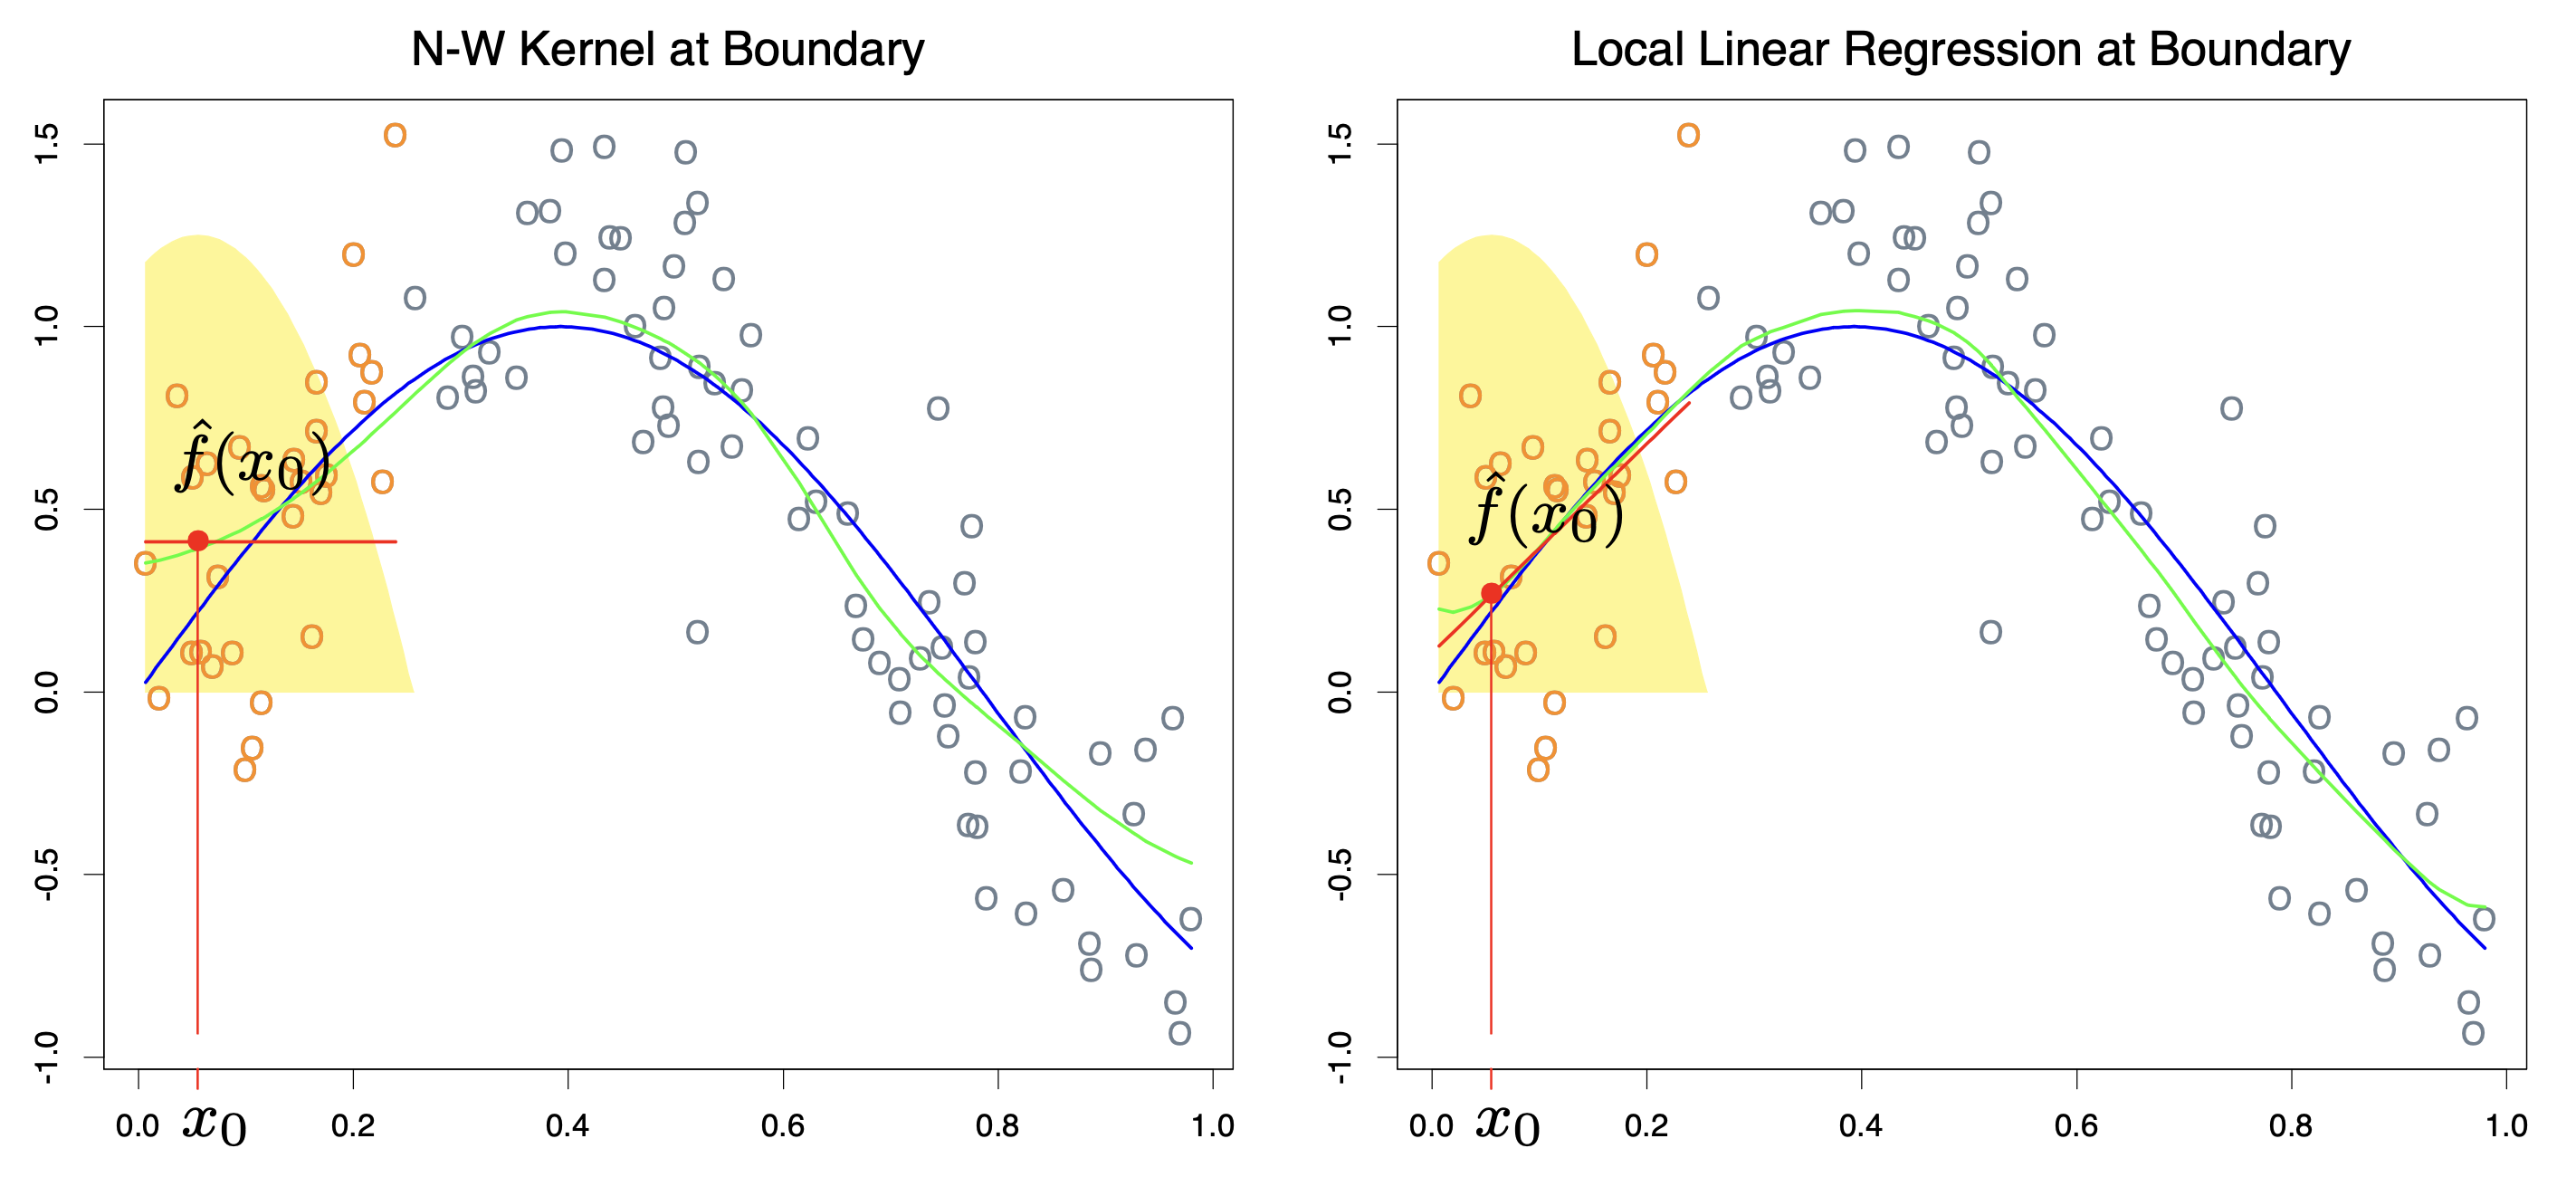
\includegraphics[width=0.78\textwidth]{images/1-28-1}
\end{figure}

Supposing $m(X_i) = \alpha + \beta x_i$, the local linear regression has 0 bias, while NW is biased for $\beta\ne 0$. This is because:
\begin{itemize}
	\item LLR tracks the first order Taylor expansion, accounting for smoothness in that $m$ is approximately linear near $x_0$.
	\item NW models $m(x) \approx m(x_0)$.\boxednote{So why use NW if LLR is over a larger class of functions?} 
	\item In fact, putting $\beta=0$ into LLR recovers NW, in that \[
		\min_\alpha \frac{1}{n} \sum\limits_{i=1}^{n} K\left( \frac{X_i-x_0}{h}\right)\left( Y_i - \alpha \right) 
	\] gives $\hat{m}(x_0) = \hat{\alpha}$.
\end{itemize}

If we redid our previous analysis, replacing NW by local linear regression, we would get in the interior
\[
		\begin{aligned}
			\MSE\left( \hat{m}(x_0) \mid X_{1:n} \right)
			&= \frac{1}{nh} \frac{\sigma^2(x_0)}{f(x_0)} \int_{-1}^{1} K^2(u)du \\
			&\quad + h^4 \left( \frac{m''(x_0)}{2} \right)^2 \left( \int_{-1}^{1} u^2K(u) du  \right)^2 \left( 1 + o_\P(1) \right)
		\end{aligned}
	,\]
so LLR gets the same rate as NW in the interior but without the design bias term of $m'(x_0) \frac{f'(x_0)}{f(x_0)}$.
At the boundary, we would have
\[
	\MSE\left( \hat{m}(0) \mid X_{1:n} \right) = \left(\frac{1}{nh} \frac{\sigma^2(0)}{f(0)} C_1(K) + h^4 m''(0)^2 C_2(K)\right) \left( 1 + o_\P(1) \right)
,\]
so there is no additional bias at the boundary compared to the interior.
We get fast MSE decay without needing kernel carpentry.\footnote{Also called automatic kernel carpentry.}

\begin{remark}[Interpolation]
	We say that $\hat{m}$ interpolates the data if $\hat{m}(X_i) = Y_i$ for all $i$.

	The traditional view is that if $\hat{m}$ interpolates the data, it overfits and is a bad estimator. Does this contradict NW? No, because we can have $K$ with a large bump at $0$.
\end{remark}

\begin{comment}
\section{Linear Smoothers}

Recall LLR solves \[
	\left( \hat{\alpha}, \hat{\beta} \right) = \argmin_{(\alpha,\beta)} \sum\limits_{i=1}^{n} K\left( \frac{X_i-x_0}{h} \right) \left( Y_i - \alpha - \beta(X_i-x_0) \right)^2
.\] Writing \[
	W = \begin{pmatrix}
		K\left( \frac{X_1-x_0}{h} \right) & \cdots & 0 \\
		0 &\ddots & 0 \\
		0 & 0 & K\left( \frac{X_n - x_0}{h} \right)
	\end{pmatrix}, \quad \tilde{X} = \begin{pmatrix}
	1 & X_1-x_0 \\
	\vdots & \vdots \\
	1 & X_n - x_0
	\end{pmatrix} , \quad Y = \begin{pmatrix}
	Y_1 \\
	\vdots \\ Y_n
	\end{pmatrix},\] we get \[
		\begin{pmatrix}
	   \hat{\alpha} \\
		\hat{\beta}
		\end{pmatrix} = \left( \tilde{X}^T W X \right)^{-1} \tilde{X}^T WY = \left\|W^{\frac{1}{2}} \left( Y - \tilde{X} \begin{pmatrix}
		\alpha \\
		0
		\end{pmatrix} 	\right) \right\|_2^{2}
	,\] \boxednote{\texthl{check}}when $\tilde{X}^T W X$ is invertible.

Thus $\hat{m}(x_0) := \hat{\alpha}=  \sum_{i=1}^{n} \gamma_i Y_i$ where $\gamma_i$ is a function of $X_{1:n}$ and $x_0$.
\end{comment}
